% !TeX root = induction-he.tex

\chapter{%
מודלים חישוביים%
}\label{s.models}

מודלים חישוביים, כגון אוטומטים סופיים ושפות פורמליות, הם מושגים מרכזיים במדעי המחשב. הוכחות בנושאים אלה משתמשות באינדוקציה מעל המבנה של אוטומט או מעל לגזירה של מחרוזות מדקדוק פורמלי. לעתים יש יותר מטענת בסיס אחת וצעד אינדוקציה אחד.

אנו מניחים שהקורא בקיא במושגים של אוטומט לא-דטרמיניסטי סופי
\L{\small NFA},
ביטוי רגולרי
\L{\small RE},
ודקדוק חסר-הקשר.


\section{%
אוטומטים%
}


\begin{theorem}
יהי
$r$
ביטוי רגולרי. אזי ניתן לבנות
\L{\small NFA}
שמקבל את השפה של
$r$.
\end{theorem}

\textbf{הוכחה}
יש שלוש טענות בסיס:
\begin{itemize}
\item $r$
הוא הקבוצה הריקה
$\emptyset$. 
ה-%
\L{\small NFA}
עם מצב תחילי אחד ומצב סופי אחד וללא מעברים לא מקבל אף מחרוזת:
\begin{center}
\selectlanguage{english}
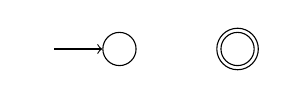
\begin{tikzpicture}[circle]
\node (dummy) at (-1,0) {};
\node (initial) at (0,0) [draw,minimum size=12pt] {};
\node (final) at (1.5,0) [draw,minimum size=15pt] {};
\node at (1.5,0) [draw,minimum size=12pt] {};
\draw[->] (dummy) -- (initial);
\end{tikzpicture}
\end{center}
\item $r$
הוא המחרוזת הריקה
$\epsilon$.
ה-%
\L{\small NFA}
עם מצב אחד שהוא גם תחילי וגם סופי מקבל את המחרוזת הריקה:
\begin{center}
\selectlanguage{english}
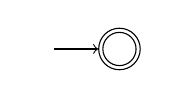
\begin{tikzpicture}[circle]
\node (dummy) at (-1,0) {};
\node (final) at (0,0) [draw,minimum size=15pt] {};
\node at (0,0) [draw,minimum size=12pt] {};
\draw[->] (dummy) -- (final);
\end{tikzpicture}
\end{center}
\item $r$
הוא התו הבודד
$a$.
ה-%
\L{\small NFA}
שלהלן מקבל את השפה
$\{a\}$:
\begin{center}
\selectlanguage{english}
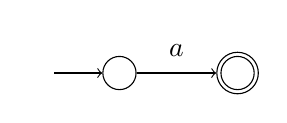
\begin{tikzpicture}[circle]
\node (dummy) at (-1,0) {};
\node (initial) at (0,0) [draw,minimum size=12pt] {};
\node (final) at (1.5,0) [draw,minimum size=15pt] {};
\node at (1.5,0) [draw,minimum size=12pt] {};
\draw[->] (dummy) -- (initial);
\draw[->] (initial) -- node[above] {$a$} (final);
\end{tikzpicture}
\end{center}
\end{itemize}

יש שלושה צעדי אינדוקציה, אחד לכל דרך לבניית
\L{\small RE}
מ-%
\L{\small REs}
פשוטים יותר:
\begin{itemize}
\item
שירשור
$r_1r_2$:
לפי הנחת האינדוקציה קיימים
\L{\small NFAs}
$\mathit{nfa}_1$
ו-%
$\mathit{nfa}_2$
המקבלים את השפות של
$r_1$
ו-%
$r_2$,
בהתאמה. בנה
$\mathit{nfa}_{12}$
על ידי הוספת מעבר ריק מהמצב הסופי של 
$\mathit{nfa}_1$
למצב התחילי של
$\mathit{nfa}_2$.
המצב התחילי של
$\mathit{nfa}_{12}$
הוא המצב התחילי של
$\mathit{nfa}_1$
והמצב הסופי שלו הוא המצב הסופי של
$\mathit{nfa}_2$:
\begin{center}
\selectlanguage{english}
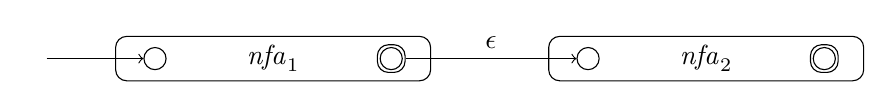
\begin{tikzpicture}[rounded corners]
\node (dummy) at (-3,0) {};
\node at (0,0) [draw,rectangle,minimum width=4cm,minimum height=.5cm] {$\mathit{nfa}_1$};
\node (initial) at (-1.5,0) [draw,minimum size=8] {};
\node (final1) at (1.5,0) [draw,minimum size=10pt] {};
\node at (1.5,0) [draw,minimum size=8] {};
\node at (5.5,0) [draw,rectangle,minimum width=4cm,minimum height=.5cm] {$\mathit{nfa}_2$};
\node (initial2) at (4,0) [draw,minimum size=8] {};
\node at (7,0) [draw,minimum size=10pt] {};
\node at (7,0) [draw,minimum size=8] {};
\draw[->] (dummy) -- (initial);
\draw[->] (final1) -- node[above] {$\epsilon$} (initial2);
\end{tikzpicture}
\end{center}

\item
איחוד
$r_1+r_2$:
לפי הנחת האינדוקציה קיימים
\L{\small NFAs}
$\mathit{nfa}_1$
ו-%
$\mathit{nfa}_2$
המקבלים את השפות של
$r_1$
ו-%
$r_2$,
בהתאמה. בנה
$\mathit{nfa}_{12}$
על ידי הוספת מצב תחילי ומצב סופי חדשים ומעברים ריקים:
\begin{center}
\selectlanguage{english}
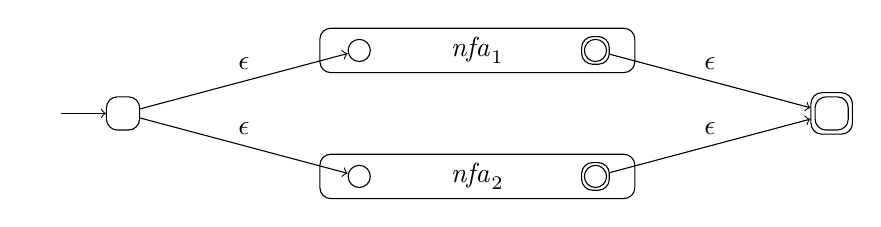
\begin{tikzpicture}[minimum size=12pt,rounded corners]
\node (initial) at (-2,0) [draw] {};
\node (final) at (7,0) [draw,minimum size=15pt] {};
\node at (7,0) [draw] {};
\node (dummy) at (-3,0) {};
\node at (2.5,.8) [draw,rectangle,minimum width=4cm,minimum height=.5cm] {$\mathit{nfa}_1$};
\node at (2.5,-.8) [draw,rectangle,minimum width=4cm,minimum height=.5cm] {$\mathit{nfa}_2$};
\node (top-initial) at (1,.8) [draw,minimum size=8] {};
\node (top-final) at (4,.8) [draw,minimum size=10pt] {};
\node at (4,.8) [draw,minimum size=8] {};
\node (bottom-initial) at (1,-.8) [draw,minimum size=8] {};
\node (bottom-final) at (4,-.8) [draw,minimum size=10pt] {};
\node at (4,-.8) [draw,minimum size=8] {};
\draw[->] (dummy) -- (initial);
\draw[->] (initial) -- node[above] {$\epsilon$} (top-initial);
\draw[->] (initial) -- node[above] {$\epsilon$} (bottom-initial);
\draw[->] (top-final) -- node[above] {$\epsilon$} (final);
\draw[->] (bottom-final) -- node[above] {$\epsilon$} (final);
\end{tikzpicture}
\end{center}

\item 
סגור
$r^*$:
לפי הנחת האינדוקציה קיים 
\L{\small NFA}
$\mathit{nfa}_r$
המקבל את השפה של
$r$.
הוסף מצב תחילי, מצב סופי ומעברים ריקים כפי שהם מוצגים בתרשים:
\begin{center}
\selectlanguage{english}
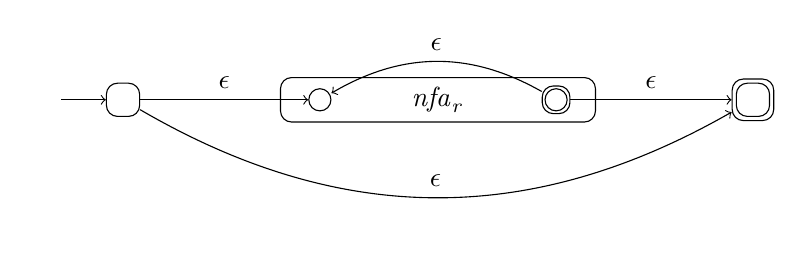
\begin{tikzpicture}[minimum size=12pt,rounded corners]
\node (initial) at (0,0) [draw] {};
\node (final) at (8,0) [draw,minimum size=15pt] {};
\node at (8,0) [draw] {};
\node (initial1) at (2.5,0) [draw,minimum size=8] {};
\node (final1) at (5.5,0) [draw,minimum size=10pt] {};
\node at (5.5,0) [draw,minimum size=8] {};
\draw[->] (final1) to [bend right=30] node[above] {$\epsilon$} (initial1);
\node (dummy) at (-1,0) {};
\node at (4,0) [draw,rectangle,minimum width=4cm,minimum height=.5cm] {$\mathit{nfa}_r$};
\draw[->] (dummy) -- (initial);
\draw[->] (initial) -- node[above] {$\epsilon$} (initial1);
\draw[->] (final1) -- node[above] {$\epsilon$} (final);
\draw[->] (initial) to [bend right=30] node[above] {$\epsilon$} (final);
\end{tikzpicture}
\end{center}
המעבר הריק בין המצב התחילי והמצב הסופי הוא עבור מחרוזת המתקבלת מאפס מופעים של
$r$,
והמעבר הפנימי מהמצב הסופי של
$\mathit{nfa}_r$
למצב התחילי שלו הוא עבור חזרה אחת או יותר של
$r$.
\end{itemize}
\qedd{5}

\section{%
שפות פורמליות%
}

הוכחות בשפות פורמליות הן באינדוקציה מעל לאורך המחרוזות, שהיא בעצם אינדוקציה מעל לגזירת המחרוזת מהדקדוק. הנה דקדוק חסר-הקשר
$G$:

\begin{displaymath}
\begin{array}{l@{\hspace{2em}}l@{\hspace{2em}}l@{\hspace{2em}}l}
S \rightarrow aB & S \rightarrow bA & A \rightarrow a & B \rightarrow b \\
A \rightarrow aS & B \rightarrow bS & A \rightarrow bAA & B \rightarrow aBB\\
\end{array}
\end{displaymath}

\begin{theorem}
השפה
$L$
של הדקדוק
$G$
היא כל המילים מעל
$\{a,b\}$
עם מספר שווה של
$a$
ו-%
$b$.
סימון:
\begin{displaymath}
S \stackrel{*}{\Rightarrow} w \;\;\mathrm{iff}\;\; \#a = \#b,
\end{displaymath}
כאשר
$\#a,\#b$
מסמנים את מספר ה-%
$a$
וה-%
$b$
ב-%
$w$.
\end{theorem}

\textbf{הוכחה}
נשתמש באינדוקציה
\textbf{בו-זמנית}
על שלוש הטענות האלו:
\begin{eqnarray}
S \stackrel{*}{\Rightarrow} w &\;\;\mathrm{iff}\;\;& \#a = \#b\label{eq.formal1}\\
A \stackrel{*}{\Rightarrow} w &\;\;\mathrm{iff}\;\;& \#a = \#b+1\label{eq.formal2}\\
B \stackrel{*}{\Rightarrow} w &\;\;\mathrm{iff}\;\;& \#a+1 = \#b.\label{eq.formal3}
\end{eqnarray}
טענת הבסיס
$|w|=1$
פשוטה כי
$A$
ו-%
$B$
גוזרים את
$a$
ו-%
$b$,
בהתאמה, ו-%
$S$
לא גוזר אף מחרוזת באורך אחד. עלינו לציין שאין דרכים אחרות לקבל מחרוזת באורך אחד.

תהי 
$w$
מילה הנגזרת מ-%
$S$
עם 
$|w|=n+1$.
יש שלושה צעדי אינדוקציה וכדי להוכיח כל אחד מהם נניח את
\textbf{כל שלוש הטענות}
עבור 
$|w|=n$
כהנחת האינדוקציה.

תחילה נוכיח את הנוסחה
\ref{eq.formal1}
עבור
$w$.
הגזירה הראשונה היא אחת מ:
\[
S\rightarrow aB \stackrel{*}{\Rightarrow} aw',\hspace{3em} S\rightarrow bA\stackrel{*}{\Rightarrow} bw'\,.
\]
במקרה הראשון, לפי הנחת האינדוקציה בנוסחה
\ref{eq.formal3},
עבור המילה
$w'$ 
שנגדרה על ידי
$B$
קיים
$\#a+1=\#b$,
כך ש-%
$\#a=\#b$
ב-%
$w$.
בדרך דומה ניתן להוכיח את המקרה השני תוך שימוש בנוסחה~
\ref{eq.formal2}.

נשאיר את סיום ההוכחה כתרגיל.
\qed

\begin{exercise}\mbox{}
\begin{itemize}
\item
הוכח את הנוסחאות
\ref{eq.formal2}
ו-%
\ref{eq.formal3}.
\item
הוכח את המשפט ההפוך: אם
$\#a=\#b$
ב-%
$w$
אזי
$S \stackrel{*}{\Rightarrow} w$.
\end{itemize}
\end{exercise}

%%%%%%%%%%%%%%%%%%%%%%%%%%%%%%%%%%%%%%%%%%%%%%%%%%%%%%%%%%%%%%%%%%%
